\section{Application} \label{sec:application}
In this section, we will cover the implemented benchmark application in detail.
The code is available on Github\footnote{https://github.com/silvanheller/parquet-demo}

\subsection{Technologies used}
Our benchmarking application uses Apache Spark\footnote{http://spark.apache.org/} as Queryengine.
The programming language used is Scala\footnote{https://www.scala-lang.org/}.
We compare Parquet to JSON, CSV and Apache ORC\footnote{https://orc.apache.org/}

\subsection{Scenario I - Column Storage}
\label{sec:scenario-one}
Scenario I is intended to showcase the power of columnar storage formats.
It features a table schema with a lot of columns, only one of which is accessed for the given query.
The other columns are filled with strings, given that today's data sets often feature highly varied and unstructured data.

\subsubsection{Table Layout}
Given a number of rows $n_rows$, a number of columns $n_cols$ and the length of a string $s_length$, the table schema is depicted in Table \ref{table:schema-one}
\begin{table}[h]
\centering
\caption{Table Layout for Scenario 1}
\label{table:schema-one}
\renewcommand{\arraystretch}{1.4}
{\setlength{\tabcolsep}{1em}
\begin{tabular}{|c|c|c|c|c|}
\hline
id      & data1                & data2                & ... & data{[}n\_cols{]}    \\ \hline
1       & rand\_string(s\_len) & rand\_string(s\_len) & ... & rand\_string(s\_len) \\ \hline
...     & ...                  & ...                  & ... & ...                  \\ \hline
n\_rows & rand\_string(s\_len) & rand\_string(s\_len) & ... & rand\_string(s\_len) \\ \hline
\end{tabular}}
\end{table}

\subsubsection{Query}
\label{sec:query-one}
The query we have chosen for this scenario is a simple average over the 'id' column.
Code-snippet \ref{code:scenario1-avg-spark} shows how this is done in Scala and snippet \ref{code:scenario1-avg-sql} shows the equivalent SQL query.
\begin{lstlisting}[language=Scala,caption=Average over the ID Column in Spark, label=code:scenario1-avg-spark, captionpos=b]
def getAVG(df: DataFrame): DataFrame = {
  df.agg(avg("id"))
}
\end{lstlisting}
\begin{lstlisting}[language=SQL,caption=Equivalent SQL Query, label=code:scenario1-avg-sql, captionpos=b]
  SELECT AVG(id) FROM table;
\end{lstlisting}
This requires acessing all rows and prevents automatically created index structures such as in ORC from interfering with our measurements.
Apache Spark uses lazy evaluation for queries, which enables us to read the data from cold storage.
This also means queries are run only once on the dataset since afterwards the data might be cached somewhere.

\subsection{Scenario II - Nested Object Storage}
Scenario II is designed to benchmark nested object storage.
As discussed in Section \ref{section:parquet-nested}, parquet stores nested objects by creating separate tables per attribute.

\subsubsection{Table Layout}

Our Table is a collection of $Persons$. Each Person has a name and an age, two Parents, which in turn have Parents (Four Grandparents).
Each Grandparent is a successor of Adam (inspired by Christian Mythology). Graphically, our Schema is represented in Figure \ref{fig:schema-scenario2}

\begin{figure}[h]
\centering
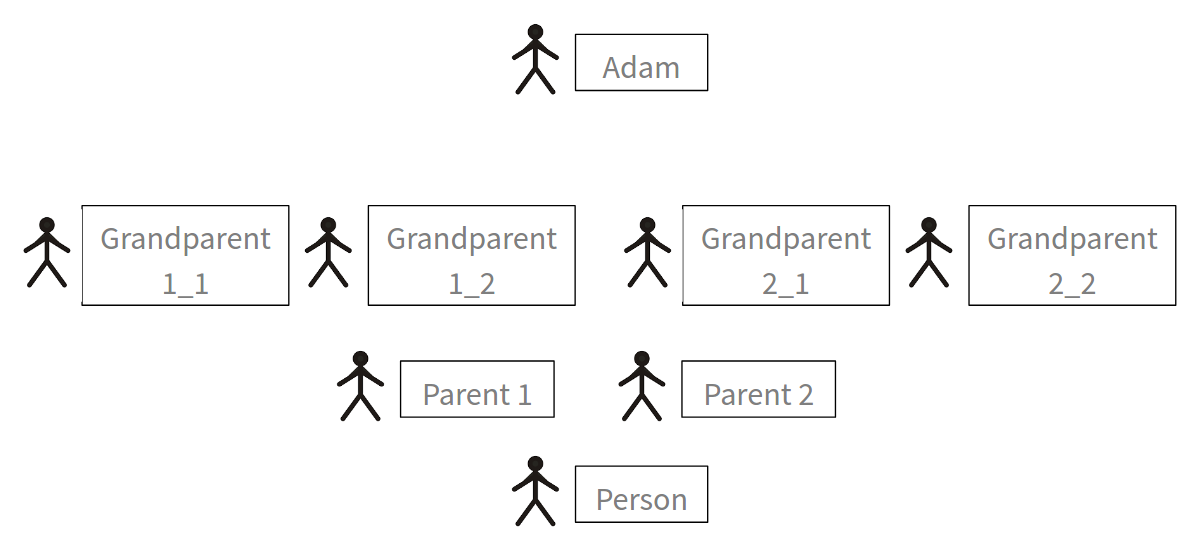
\includegraphics[width=0.8\textwidth]{schema-scenario2.png}
\caption{Scenario 2 visualized}
\label{fig:schema-scenario2}
\end{figure}

For Parquet, this results in 2 (person-columns)+ 4 (parent-columns) + 8 (grandparent-columns) + 8 (adam-columns) = 22 tables.
In the interest of readability, we will not list them all.
%They are: \\
%$person.name$, $person.age$, \\
%$person.parent1.name$, $person.parent1.age$, \,$person.parent2.name$,\, $person.parent2.age$, \\
%$person.parent1.grandparent1_1.name$, $person.parent1.grandparent1_1.age$, $person.parent1.grandparent1_2.name$, $person.parent1.grandparent1_2.age$, \\
%$person.parent2.grandparent2_1.name$, $person.parent2.grandparent2_1.age$, $person.parent2.grandparent2_2.name$, $person.parent2.grandparent2_2.age$, \\
%$person.parent1.grandparent1_1.adam.name$, $person.parent1.grandparent1_1.adam.age$, $person.parent1.grandparent1_2.adam.name$, $person.parent1.grandparent1_2.adam.age$, \\
%$person.parent2.grandparent2_1.adam.name$, $person.parent2.grandparent2_1.adam.age$, $person.parent2.grandparent2_2.adam.name$, $person.parent2.grandparent2_2.adam.age$, \\
\subsubsection{Queries}

Again, we average over a column. This time, we have chosen the $person.parent1.grandparent1\_1.adam$ column.

Code-snippet \ref{code:scenario1-avg-spark} shows how this is done in Scala and snippet \ref{code:scenario1-avg-sql} shows the equivalent SQL query.
\begin{lstlisting}[language=Scala,caption=Average over the ID Column in Spark, label=code:scenario1-avg-spark, captionpos=b]
def getAVG(df: DataFrame): DataFrame = {
  df.agg(avg("parent1.grandparent1_1.adam.age").as("adamage"))
}
\end{lstlisting}
\begin{lstlisting}[language=SQL,caption=Equivalent SQL Query, label=code:scenario1-avg-sql, captionpos=b]
  SELECT AVG(parent1.grandparent1_1.adam.age) FROM table;
\end{lstlisting}

The same considerations as with Scenario I apply when choosing the query.